\section{Integrarea DVM cu comutatorul software LINC: \textit{LINC-WE}}

Așa cum a fost descris anterior, simulatorul \gls{dvm} permite emularea nivelului mediator care apare în arhitectura \gls{sdn} a rețelelor de transport de date fără fir. Se pot simula diferite topologii de rețea prin manipularea fişierelor \gls{xml} de configurare ale diferitelor instanţe ale \gls{dvm}, făcând simulatoarele să prezinte diferite configuraţii. Această abordare oferă un bun prim pas pentru simularea rețelelor de transport de date fără fir în contextul \gls{sdn}, însă nu este suficient, deoarece instanţele \gls{dvm} sunt independente și rețeaua simulată nu este completă, deoarece nu există legături între dispozitivele simulate. Din acest motiv, această secţiune prezintă încercarea de a integra simulatorul \gls{dvm} cu un comutator software deja existent, care a fost folosit anterior pentru simulări de rețele optice în contextul \gls{sdn}: \textit{Legătura Nu Este Închisă} - \gls{linc} și cu simulatorul de rețele definite prin software, \textit{mininet}. Comutatorul software folosit anterior în simularea rețelelor optice~\cite{parulkar2015sdn, kretsis2016emulation, mehmeri2017software}, bazat pe \gls{linc} se numeşte \textit{Legătura Nu Este Închisă - Extensii Optice} - \gls{linc-oe}, astfel că am denumit comutatorul rezultat în urma integrării \gls{dvm} cu \gls{linc}: \textit{Legătura Nu Este Închisă - Emulator Fără Fir} - \gls{linc-we}~\cite{stancu2017wireless}.

\subsection{LINC}

\gls{linc} este un comutator software ce suportă protocolul OpenFlow, scris în limbajul de programare Erlang~\cite{lincsw}. A fost proiectat să fie modular, oferind o metodă rapidă de a face prototipuri \gls{sdn} și de a testa noi caracteristici ale protocolului OpenFlow. Este oferit ca o implementare cu sursă deschisă de către \textit{FlowForwarding.org} și are ca scop oferirea unei soluții prin care utilizatorii pot evalua rapid protocoalele OpenFlow și OF-Config.

Un singur comutator este implementat ca un nod Erlang și cuprinde mai multe comutatoare logice. Acestea, porturile și legăturile dintre porturi sunt descrise de către utilizator prin intermediul unui fișier de configurare, așa cum este ilustrat și în Figura \ref{fig:linc_architecture}. Datorită acestei arhitecturi modulare, comutatorul \gls{linc} este capabil să ofere mai multe implementări pe care utilizatorul le poate alege, fiecare având asociată o versiune diferită a protocolului OpenFlow (versiunile 1.2, 1.3 sau 1.4). Aceste implementări sunt responsabile de comutarea pachetelor și alterarea tabelelor de fluxuri de date.

\begin{figure}[h]
	\centering
	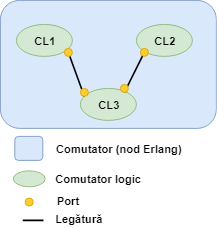
\includegraphics{linc_architecture}
	\caption{Arhitectura comutatorului software LINC~\cite{linc2014qsg}.}
	\label{fig:linc_architecture}
\end{figure}

După cum este prezentat în~\cite{linc2014qsg}, \gls{linc} prezintă mai multe blocuri software: comutatorul capabil OpenFlow, modului protocolului OpenFlow, modului protocolului OF-Config. Acestea sunt dezvoltate ca aplicații Erlang separate, respectând principiile \textit{Platforma Telecom Deschisă} - \gls{otp} ale limbajului Erlang. Există și o componentă separată care se ocupă de conexiunea la un echipament de control \gls{sdn}. Tabelele de fluxuri, porturile sau tabelele de grup sunt administrate de implementările separate reprezentând diferitele versiuni ale protocolului OpenFlow.

\subsubsection{LINC-OE}

Datorită naturii modulare a comutatorului \gls{linc}, a apărut o nouă implementare care să acopere cazurile de utilizare ale \gls{sdn} din domeniul optic: \gls{linc-oe}. Acesta reprezintă un simulator de comutatoare optice care suportă extensiile optice ale protocolului OpenFlow. Diferenţa dintre \gls{linc} și \gls{linc-oe} este că, în cazul celui din urmă, comutatoarele logice care sunt simulate reprezintă comutatoare optice, astfel că spre deosebire de interfeţele electrice, porturile optice oferă mai multe canale de comunicaţie independente, diferenţiate prin lungimea de undă. În implementarea \gls{linc-oe}, mesajele ce se transmit printr-un astfel de port optic nu mai sunt pachete Ethernet, ci mesaje Erlang, ce conţin informații adiţionale, pe lângă pachetul Ethernet propriu-zis. O altă diferenţă este dată de faptul ca \gls{linc-oe} oferă interfețe pentru simularea defectării legăturilor dintre porturi.

\subsubsection{Interfaţa NETCONF}

Comutatorul software \gls{linc} expune de asemenea și o interfață \gls{netconf}. Este folosită de către protocolul OF-Config și este disponibilă pentru un comutator doar dacă acel protocol este folosit. În cazul în care este permisă utilizarea acestuia, o nouă aplicație Erlang este pornită în cadrul nodului Erlang: \textit{enetconf}, care pornește un server \gls{netconf} ce aşteaptă conexiuni pe adresa \gls{ip} și portul selectate de utilizator.

Această abordare prezintă un dezavantaj major: un singur server \gls{netconf} este pornit pentru comutatorul \gls{linc}, astfel că nu se pot accesa comutatoarele logice care alcătuiesc comutatorul \gls{linc} individual prin interfaţa \gls{netconf}. Acestea pot fi configurate doar prin intermediul protocolului OpenFlow.

De asemenea, modelul informațional \gls{yang} care este expus de către server nu este configurabil, astfel încât utilizatorul nu poate alege un model \gls{yang} pe care comutatorul software să îl poată folosi. Dacă acest lucru ar fi fost oferit, ar fi fost banală transformarea \gls{linc-oe} în \gls{linc-we}, prin înlocuirea modelului \gls{yang} expus cu modelul informațional pentru microunde și apoi corelarea atributelor \gls{yang} cu parametrii comutatorului \gls{linc}.

\subsection{LINC-WE}

\gls{linc-we} a apărut ca o încercare de a îmbunătăţi simulatorul \gls{dvm} dezvoltat anterior, prin oferirea unei soluții care să simuleze nu doar dispozitive de rețea independente, ci și legăturile dintre acestea. Astfel, am luat în considerare integrarea \gls{dvm} cu un comutator software deja existent, \gls{linc}, având în vedere și faptul că acesta a fost folosit anterior pentru simularea de rețele optice în contextul \gls{sdn}, prin \gls{linc-oe}.

Spre deosebire de \gls{linc} și \gls{linc-oe}, \gls{linc-we} nu ilustrează utilizarea protocolului OpenFlow pentru configurarea comutatorului, ci pune accent pe protocolul \gls{netconf} pentru administrarea dispozitivelor de rețea. Oferă totuşi suportul pentru protocolul OpenFlow, prin modulele \gls{linc} care implementează versiunile 1.2, 1.3 și 1.4 ale acestuia. Deoarece configurarea și administrarea dispozitivelor de transport de date fără fir a migrat de la protocolul OpenFlow (prin dezvoltarea de extensii specifice) la \gls{netconf}, așa cum demonstrează activitatea de cercetare din cadrul \gls{onf}, prin apariția modelului informațional pentru microunde, această abordare oferind mai multă flexibilitate. \gls{linc-we} încearcă să construiască pe această bază prin oferirea unui comutator software care să expune modelele \gls{yang} propuse de \gls{onf} și să poată fi folosit în simulări.

Abordarea aleasă în acest caz a fost înlocuirea aplicaţiei Erlang \textit{enetconf}, care implementa serverul \gls{netconf} pentru comutatorul software \gls{linc} cu o aplicație externă, dezvoltată în C, care să expună modelele \gls{yang} specifice rețelelor de transport de date fără fir: \gls{dvm}.

Implementarea serverului \gls{netconf} este dată de simulatorul descris anterior, \gls{dvm}. Pentru integrarea acestuia cu comutatorul software \gls{linc} am înlocuit aplicaţia Erlang ce implementa suportul pentru acest protocol, \textit{enetconf}, cu o aplicație Erlang nouă, dezvoltată în acest scop: \textit{erl\_yuma}. Aceasta se ocupă de pornirea și oprirea serverului \gls{netconf} implementat pentru \gls{dvm}, prin deschiderea unui port Erlang care va avea această sarcină. Codul acestei soluții este oferit cu sursă deschisă și poate fi găsit pe platforma GitHub~\cite{lincwe2017}.

Din punctul de vedere al echipamentului de control \gls{sdn}, acesta va comunica prin interfaţa \gls{netconf} cu \gls{dvm}, care a fost pornit anterior din mediul Erlang (prin aplicaţia \textit{erl\_yuma}). Comunicaţia dintre aplicațiile dezvoltate în Erlang și în C este administrată de către sistemul de execuţie Erlang. Din perspectiva \textit{erl\_yuma}, comunicaţia cu \gls{dvm} se face prin mesaje standard Erlang, care sunt transmise prin portul Erlang asociat acesteia. Din cealaltă perspectivă, a \gls{dvm}, comunicaţia se realizează prin fluxurile standard de intrare și de ieșire, \textit{stdin} și \textit{stdout}. O imagine de ansamblu a arhitecturii \gls{linc-we} este prezentată în Figura \ref{fig:linc_we_architecture}.

\begin{figure}[h]
	\centering
	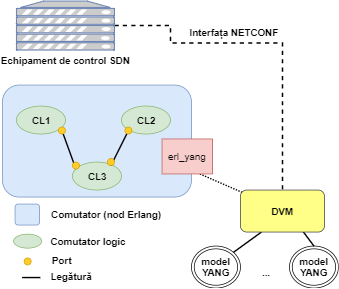
\includegraphics{linc_we_architecture}
	\caption{Arhitectura comutatorului software LINC-WE~\cite{linc2014qsg}.}
	\label{fig:linc_we_architecture}
\end{figure}

Restul arhitecturii \gls{linc} nu este influenţată: există în continuare comutatorul software, care expune o interfață \gls{netconf} (doar că acum este oferită prin \gls{dvm}) și conţine mai multe comutatoare logice, împreună cu porturile acestora și legăturile dintre ele, așa cum a fost definit în fişierul de configurare \gls{linc}. Aplicaţia ce oferă interfaţa \gls{netconf}, \textit{erl\_yuma}, este pornită doar în cazul în care protocolul OF-Config este activat.

\subsubsection{Interfața NETCONF - Aplicația Erlang}

Aplicaţia care transformă comutatorul software \gls{linc} în \gls{linc-we}, prin integrarea cu \gls{dvm} este \textit{erl\_yuma}. Aceasta este o aplicație Erlang tipică, ce respectă principiile \gls{otp}.

Structura aplicaţiei respectă recomandările \gls{otp}. În dosarul rădăcină \textit{erl\_yuma} al aplicaţiei sunt create următoarele directoare: \textit{ebin}, ce conţine fişierele compilate *.beam, dar și fişierul de resurse ale aplicaţiei \gls{otp} (ce conţine informații precum descrierea, versiunea, etc.). Directoarele \textit{include} și \textit{priv} ar trebui să conţină fişierele de incluziune *.hrl și respectiv aplicațiile externe de care depinde aplicaţia Erlang. Încă două dosare alcătuiesc aplicaţia: \textit{src}, unde se găsesc fişierele sursă și \textit{test}, ce conţine fişiere de test.

O imagine de ansamblu a aplicaţiei Erlang poate fi văzută în Figura \ref{fig:erlang_application}. Există trei fişiere sursă importante: \textit{ey\_app.erl}, \textit{ey\_sup.erl} și \textit{ey\_server.erl}.

\begin{figure}[h]
	\centering
	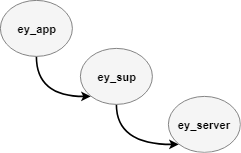
\includegraphics{erlang_application}
	\caption{Structura aplicației Erlang \textit{erl\_yuma}~\cite{linc2014qsg}.}
	\label{fig:erlang_application}
\end{figure}

Primul fişier sursă, \textit{ey\_app.erl}, reprezintă implementarea unui comportament \textit{aplicație}, așa cum este definit în \gls{otp}. Este o implementare simplă și directă a acestui comportament \gls{otp}, care oferă doar două funcții cu apel invers: \textit{start} și \textit{stop}. Prima este folosită pentru a porni procesul care este responsabil pentru implementarea aplicaţiei. Acesta este un proces \gls{otp} supervizor.

Cel de-al doilea fişier sursă, \textit{ey\_sup.erl}, implementează un comportament \textit{supervizor} definit de \gls{otp}. Acesta este procesul central al aplicaţiei \textit{erl\_yuma} și este responsabil pentru supravegherea acestuia. Este necesară implementarea unei singure funcții cu apel invers oferite de acest comportament: \textit{init}. În momentul în care procesul supervizor este pornit, această funcție este invocată, acesta fiind și locul în care ar trebui să pornim procesul \textit{ey\_server.erl}, conform cu structura aplicaţiei noaste. Nu trebuie să pornim mai multe procese copil în acest punct, deoarece dorim să expunem o singură interfață \gls{netconf}. Astfel, procesul supervizor va porni un singur modul \textit{ey\_server}.

Ultimul fişier sursă care alcătuieşte aplicaţia \textit{erl\_yuma} este \textit{ey\_server.erl}. Din punctul de vedere \gls{otp}, acest modul implementează un comportament \textit{gen\_server} (server generic). Acest proces este responsabil de crearea unui port Erlang, care porneşte aplicaţia externă C, reprezentată de \gls{dvm}. Astfel, procesul va stoca portul care a fost creat. În funcţia cu apel invers \textit{init}, practic însemnând atunci când procesul este pornit, un port Erlang este creat. Intern, acest lucru înseamnă crearea unui nou proces, bazată pe o anumită comandă. Comanda este definită ca o variabilă de mediu și este stocată în fişierul de resurse ale aplicaţiei și reprezintă de fapt comanda necesară pornirii \gls{dvm}. A fost folosită această abordare pentru a fi uşor de modificat în cazul în care comanda cu care se porneşte \gls{dvm} se va schimba pe viitor. Astfel, aplicaţia Erlang nu va trebui recompilată.

Un aspect interesant îl constituie modalitatea în care portul Erlang trebuie închis. Când utilizatorul doreşte închiderea \gls{linc-we}, trebuie ca și \gls{dvm} să fie închis, astfel încât să fie pregătit pentru o eventuală viitoare rulare. Acest lucru se face prin implementarea funcţiei cu apel invers \textit{terminate} a modulului \textit{ey\_server}. Este important de menţionat faptul că pentru ca această funcție să fie invocată în momentul închiderii aplicaţiei, aceasta trebuie să proceseze mesaje capcană (\textit{trap message}). Implementarea funcţiei \textit{terminate} va trebui să închidă instanţa \gls{dvm} care rulează (prin trimiterea unui semnal de închidere a procesului către sistemul de operare).

În prima versiune a \gls{linc-we} nu a fost implementată comunicaţia dintre aplicațiile Erlang și C. Cu ajutorul acesteia s-ar fi putut manipula parametrii comutatorului software, prin operații \gls{netconf}. Practic, \gls{linc-we} doar crează o instanţă un simulator \gls{dvm}, expunând o interfață \gls{netconf}, care însă nu implementează și modificarea atributelor comutatorului \gls{linc}.

\subsection{Concluziile integrării}

O unealtă ce oferă posibilitatea de a simula rețele ce conţin dispozitive de transport de date fără fir, care să expună și modelul informațional pentru microunde propus de \gls{onf} este importantă atât pentru membrii \gls{onf}, care pot testa, revizui și îmbunătăţi modelul, cât și pentru dezvoltatorii de aplicații \gls{sdn} care pot începe implementarea și testarea de software pentru astfel de rețele. Deoarece TR-532 a fost propus de curând, în decembrie 2016, nu există încă suport pentru acesta în simulatoare de rețea consacrate, precum OPNET sau OMNeT++, făcând \gls{linc-we} prima încercare de simulator care să ofere o astfel de interfață unui echipament de control \gls{sdn}.

\gls{linc-we} oferă posibilitatea unei lansări rapide a unui simulator ce suportă modelul TR-532 și, spre deosebire de \gls{dvm}, care era oferea doar serverul \gls{netconf} ce expunea modelele informaționale \gls{onf}, oferă și posibilitatea de a transmite trafic de date prin rețeaua simulată. Acest lucru este posibil deoarece \gls{linc-we} se bazează pe soluţia deja existentă și folosită în rețele optice, \gls{linc-oe}. Parte din cercetarea anterioară a fost și integrarea \gls{linc-oe} cu simulatorul de rețele definite prin software, \textit{mininet}, astfel că și \gls{linc-we} va fi integrat implicit cu această unealtă.

Această abordare a permis o integrare rapidă a \gls{linc} cu \gls{dvm}. După parcurgerea etapei destul de greoaie de învăţare a limbajului de programare Erlang, în care este implementat comutatorul software \gls{linc}, integrarea cu \gls{dvm} a fost facilă, aplicaţia Erlang ce se ocupă de acest aspect, descrisă anterior, fiind destul de simplă. Aceasta respectă principiile \gls{otp} și porneşte instanţa \gls{dvm} ce expune modelele \gls{yang} dorite.

Un alt avantaj oferit de această soluție este faptul că \gls{linc-we} oferă atât suport pentru protocolul \gls{netconf}, cât și pentru protocolul OpenFlow. Astfel, un echipament de control \gls{sdn} poate folosi, pe de o parte, interfaţa \gls{netconf} pentru a configura parametrii dispozitivelor simulate și, pe de altă parte, interfaţa OpenFlow pentru a administra traficul din rețea prin manipularea tabelelor de fluxuri ale echipamentelor.

Principalul dezavantaj al abordării folosite în cadrul \gls{linc-we} este faptul că poate oferi o singură interfață \gls{netconf}, care este asociată cu comutatorul software și nu câte o interfață \gls{netconf} pentru fiecare comutator logic din interiorul topologiei. Soluția evidentă ar fi pornirea câte unei aplicații \textit{erl\_yuma} pentru fiecare astfel de comutator, însă aceasta nu este banală și uşor de implementat, deoarece \gls{dvm} nu este proiectat să ruleze mai multe instanţe pe aceeaşi mașină, având anumite lucruri ce nu pot fi împărţite (de exemplu portul pe care aşteaptă conexiuni serverul \gls{netconf}, sau fişierul \gls{xml} de configurare).

Un alt dezavantaj îl constituie faptul că \gls{linc-we} nu este uşor de utilizat. Trebuie urmaţi mai mulți paşi înainte ca acesta să poată fi pornit: instalarea comutatorului software \gls{linc}, care implică instalarea mediului Erlang în prealabil; apoi, simulatorul \gls{dvm} trebuie instalat, după ce a fost instalată anterior soluţia software OpenYuma.

Fiind doar prima versiune a \gls{linc-we}, a fost implementată rapid pentru a putea fi folosită pentru teste. Asta înseamnă că se pot aduce multe îmbunătăţiri acestei soluții. Un aspect important ce ar putea fi luat în considerare este asocierea parametrilor din modelul informațional pentru microunde cu parametri reali din comutatorul software. Asta implică, însă, o înţelegere mai aprofundată a limbajului de programare Erlang. Implementarea comutatorului \gls{linc} ar putea ţine cont de aceşti parametri în simulare. De exemplu, dacă frecvenţele emiţătoarelor și receptoarelor unor porturi care comunică nu se potrivesc, comunicarea între acestea ar putea fi oprită în implementarea comutatorului.

Dată fiind dificultatea limbajului de programare Erlang și limitările descrise anterior, am renunţat la dezvoltarea unei a doua versiuni a \gls{linc-we} și am căutat o alternativă la această abordare care să fie mai facilă și mai uşor de dezvoltat și implementat. Soluția găsită a fost folosirea unei unelte de creare a unor containere software care pot rula într-un mod izolat anumite aplicații: \textit{docker}. Aceasta va fi detaliată în capitolul următor.